\documentclass[11pt]{article}
\usepackage{graphicx}
\usepackage[legalpaper,landscape, margin=0.4in]{geometry}
\usepackage{multicol}
\usepackage{titlesec}

\titlespacing*{\subsection}
{0pt}{1ex plus 1ex minus .3ex}{0ex}
\titlespacing*{\subsubsection}
{0pt}{1ex plus 1ex minus .3ex}{0ex}
\titleformat{\subsection}
  {\normalfont\fontsize{11}{15}\bfseries}{\thesection}{1em}{}
  \titleformat{\subsubsection}
  {\normalfont\fontsize{8}{15}\bfseries}{\thesection}{1em}{}
\begin{document}
\pagenumbering{None}
\setlength{\columnsep}{1cm}
\begin{multicols*}{3}
CS3245 cheatsheet
\subsection*{IR}
\textbf{Inverted index}\\
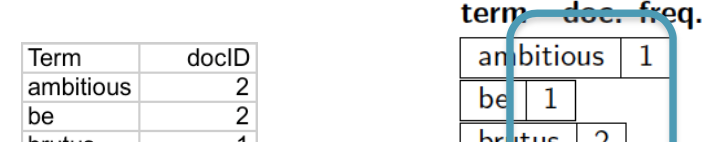
\includegraphics[height=1.5cm]{ir1}\\
Document frequency is number of times the term appear in different documents
\\
\\
\textbf{Boolean retrieval}\\
AND results in few results, OR results in many results, information overload!
\\
\textbf{Ranked retrieval}\\
query written in human language
\\
Rank each document with a score in [0, 1] which measures how well the document and query match
\\
\textbf{Bag of words}\\
doesn't consider ordering of words in document

\subsection*{Add one smoothing}
does not favor training data
\\
word with first letter capitalised is different from the word with first letter in lowercase
\\
double count add-one-smoothing maintains the counting separately, still add one but store the second count in another list
\\\\
$\mathrm{\frac{ count\ of\ term\ in\ current\ corpus\ + smoothed\ count\ of\ observed\ term}{total\ counts\ for\ all\ words\ in \ corpora + total\ smoothed\ counts\ added\ for\ terms}}$
\subsection*{Term count matrices}
Each document is a count (column) vector
\\
\subsection*{tfxidf}
\textbf{tf weight} (log frequency) 1 + $log_{10}{tf}$ if tf $>$ 0 
\\\\
\textbf{inverse document frequency}
Meant to lower the weight of more common terms and increase weight for rare terms\\
idf $\mathrm{log_{10}{(cf_{t} / df_{t}})}$
\\
\\
score will contain the weights for all terms in the q $\cap$ d
\subsection*{cosine similarity}
sum(q_{i} \ast d_{i})\\\\
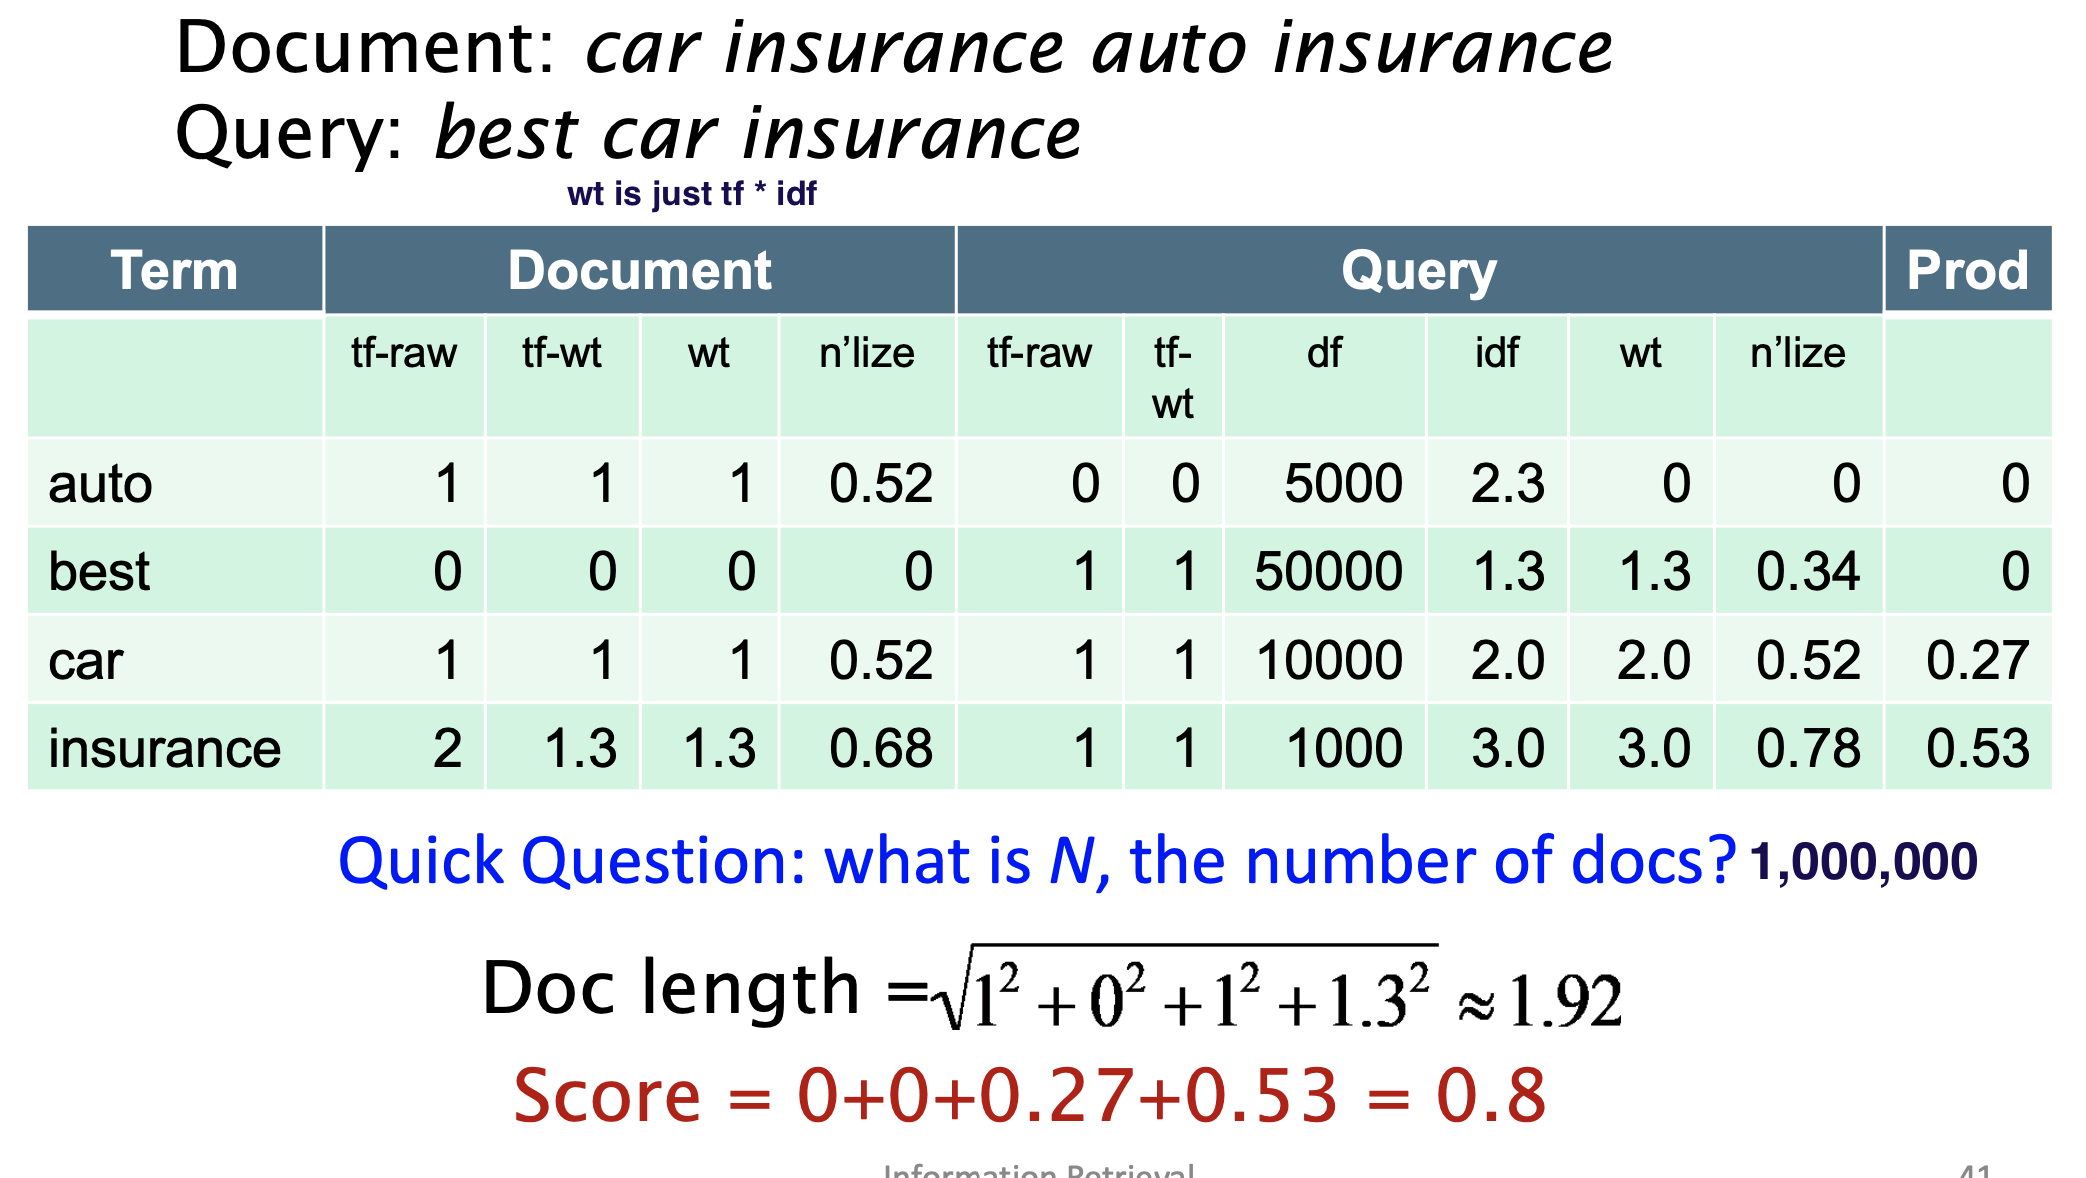
\includegraphics[height=5cm]{irl}
\subsection*{Biword index}
quiet phone call\\
2-gram\\
quiet phone, phone call
\\
False positives\\
but quiet phone can phone call may exist in different positions in the document 
False negatives cannot occur as it appears in posting list of "quiet phone" and "phone call"
and will be part of the intersection when merged and returned
\subsection*{Positional index}
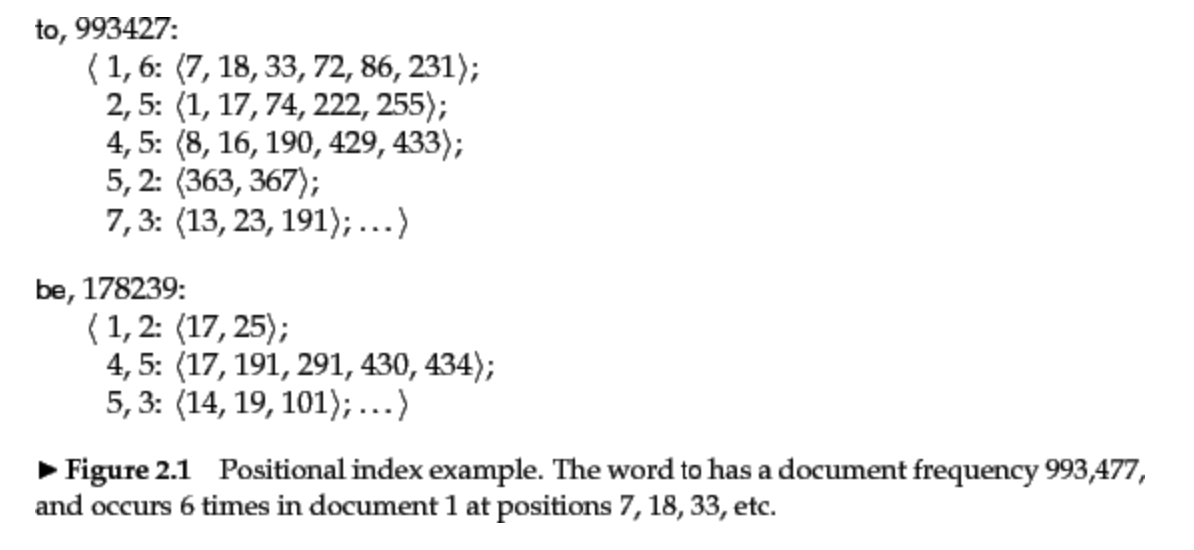
\includegraphics[height=3cm]{ir5}\\
narrow down the potential documents quickly \\
this is especially helpful when two juxtaposed query terms exist in many documents but whose intersection is small
\subsection*{Biword + Positional index}
A hybrid algorithm might first use the biword index to quickly determine the set of documents that could contain the query.
get $d_{to} \cap d_{be} $\\
Since doc 1 contains be 2 times, process doc 1\\\\
 Next, the algorithm would verify which candidate documents actually contain the phrase by checking through the positional postings. In both phases, we can use the strategy to process smaller document frequency items first. For efficiency, the biword index could also maintain the document frequency and postings pointer for its individual words, to save the cost of the additional dictionary lookups that would be incurred otherwise. 
\subsection*{Skip pointer}
skip pointer to point to end of list\\
10\\
$1 \rightarrow 2 \rightarrow 3 \rightarrow 4 \rightarrow 5$
\\\\
Dense cluster chance of skipping is high, it would be more effective to have a single skip pointer 1 \rightarrow 15\\
\\
\subsection*{Overlap measure- Jaccard coefficient}
assign number between 0 and 1
\\\\
$\frac{\| X \cap Y \|}{\| X \cup Y \| }$\\\\
for trigram Tue,ues,esd,sda,day\\ 
If both words are same, jaccard is 1\\
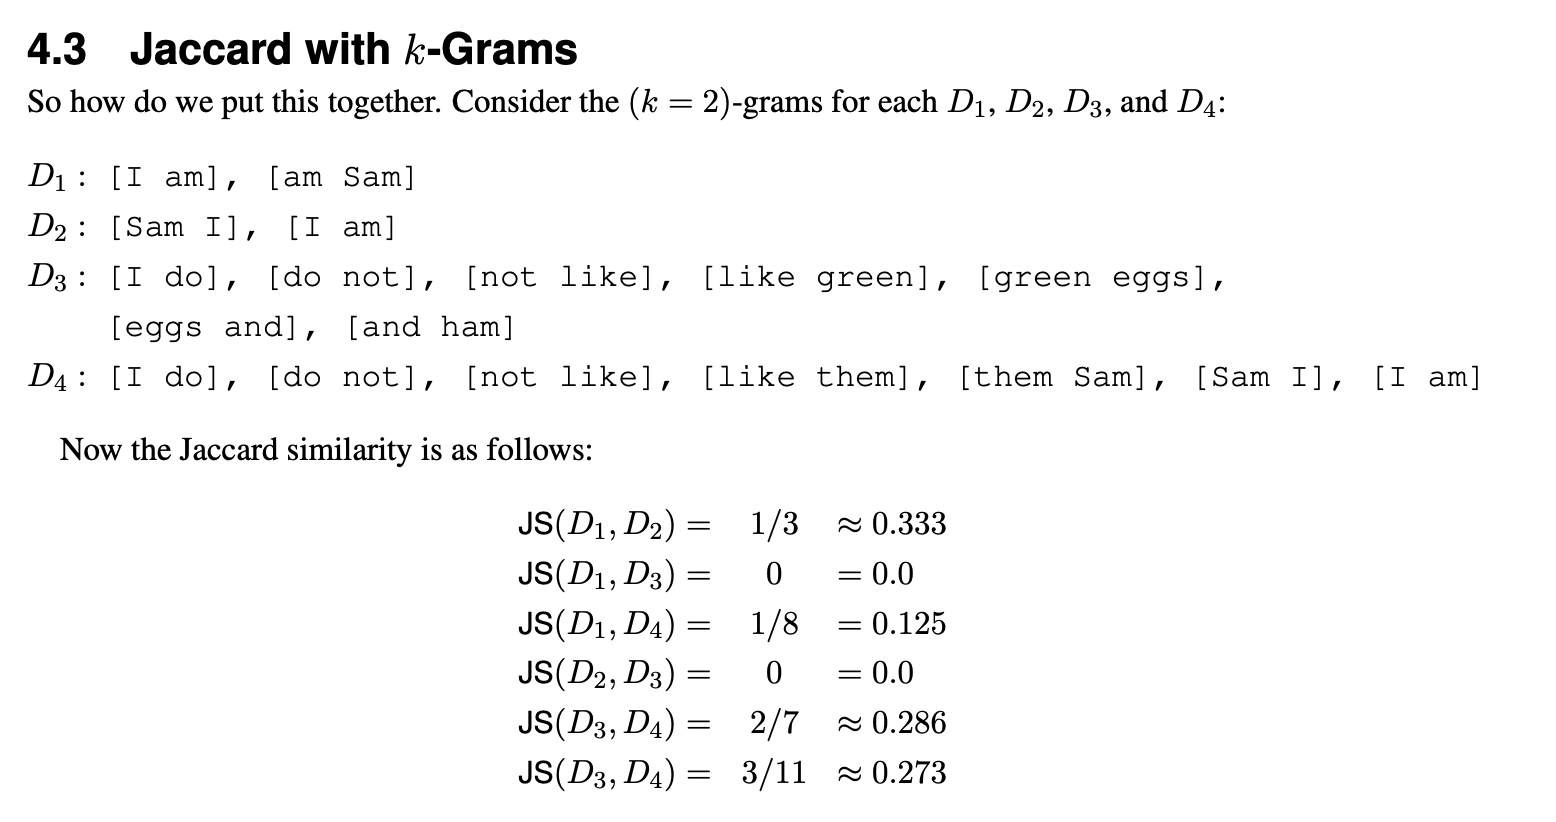
\includegraphics[height=5cm]{ir4}\\
\subsection*{Soundex}
only suitable for context of English\\
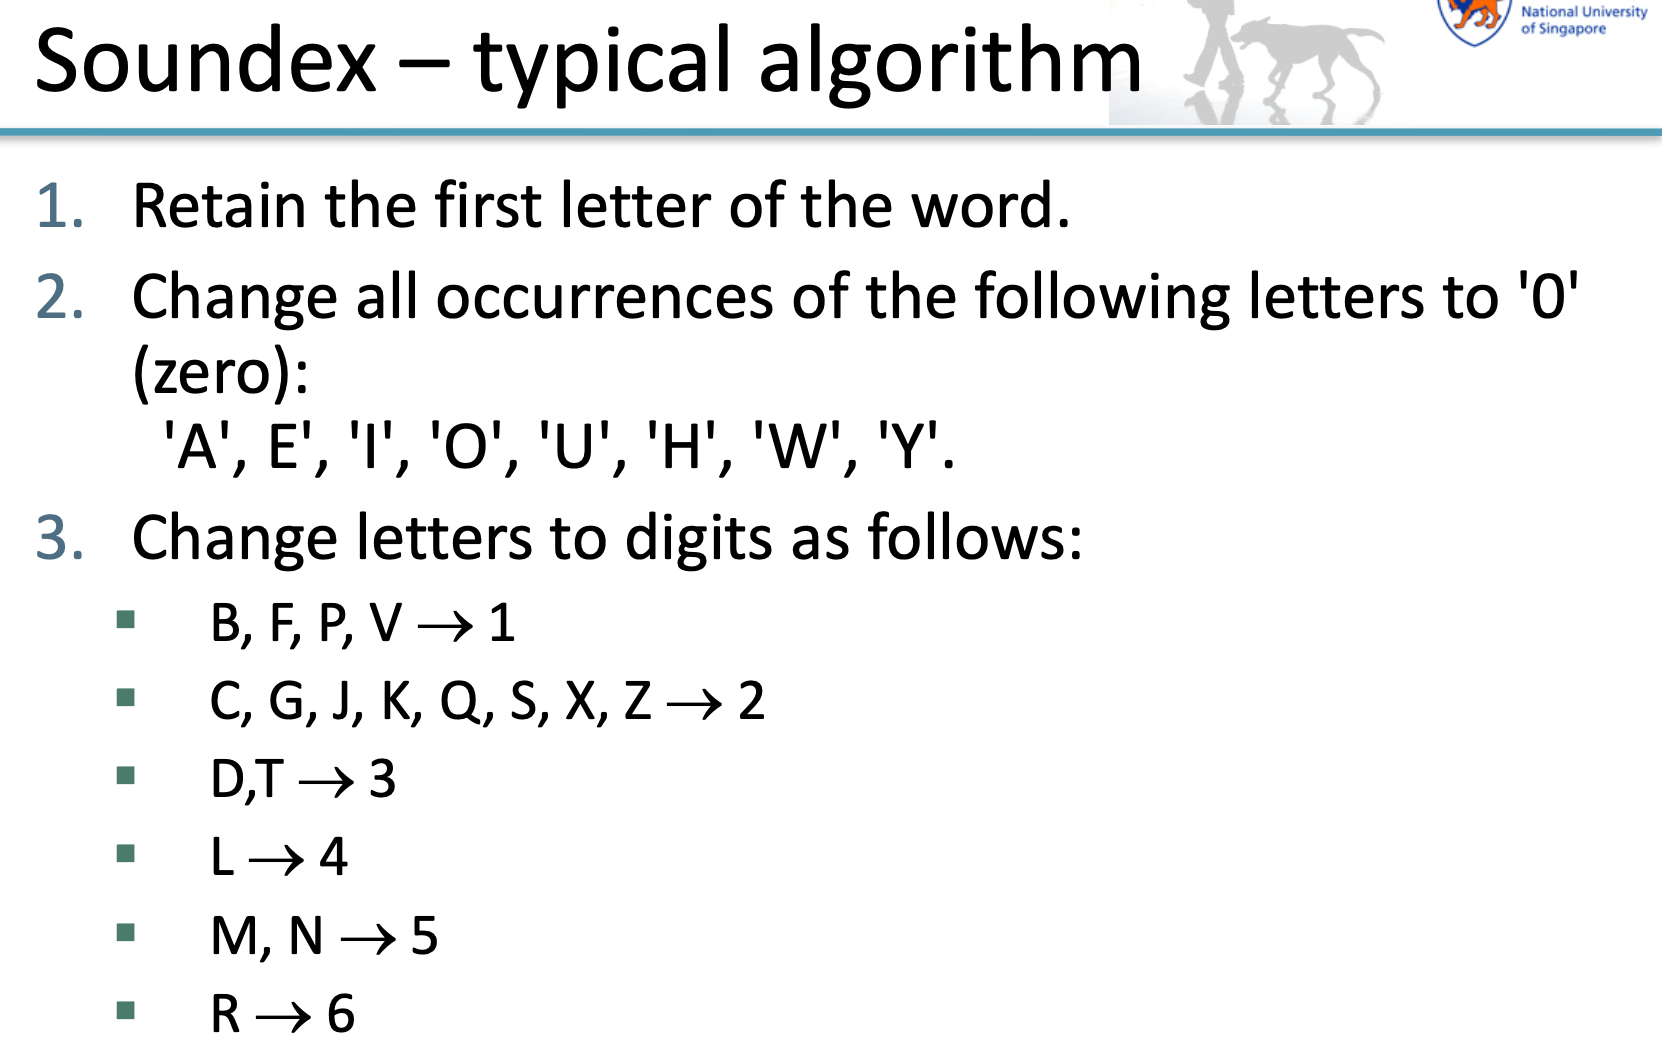
\includegraphics[height=5cm]{ir2}\\
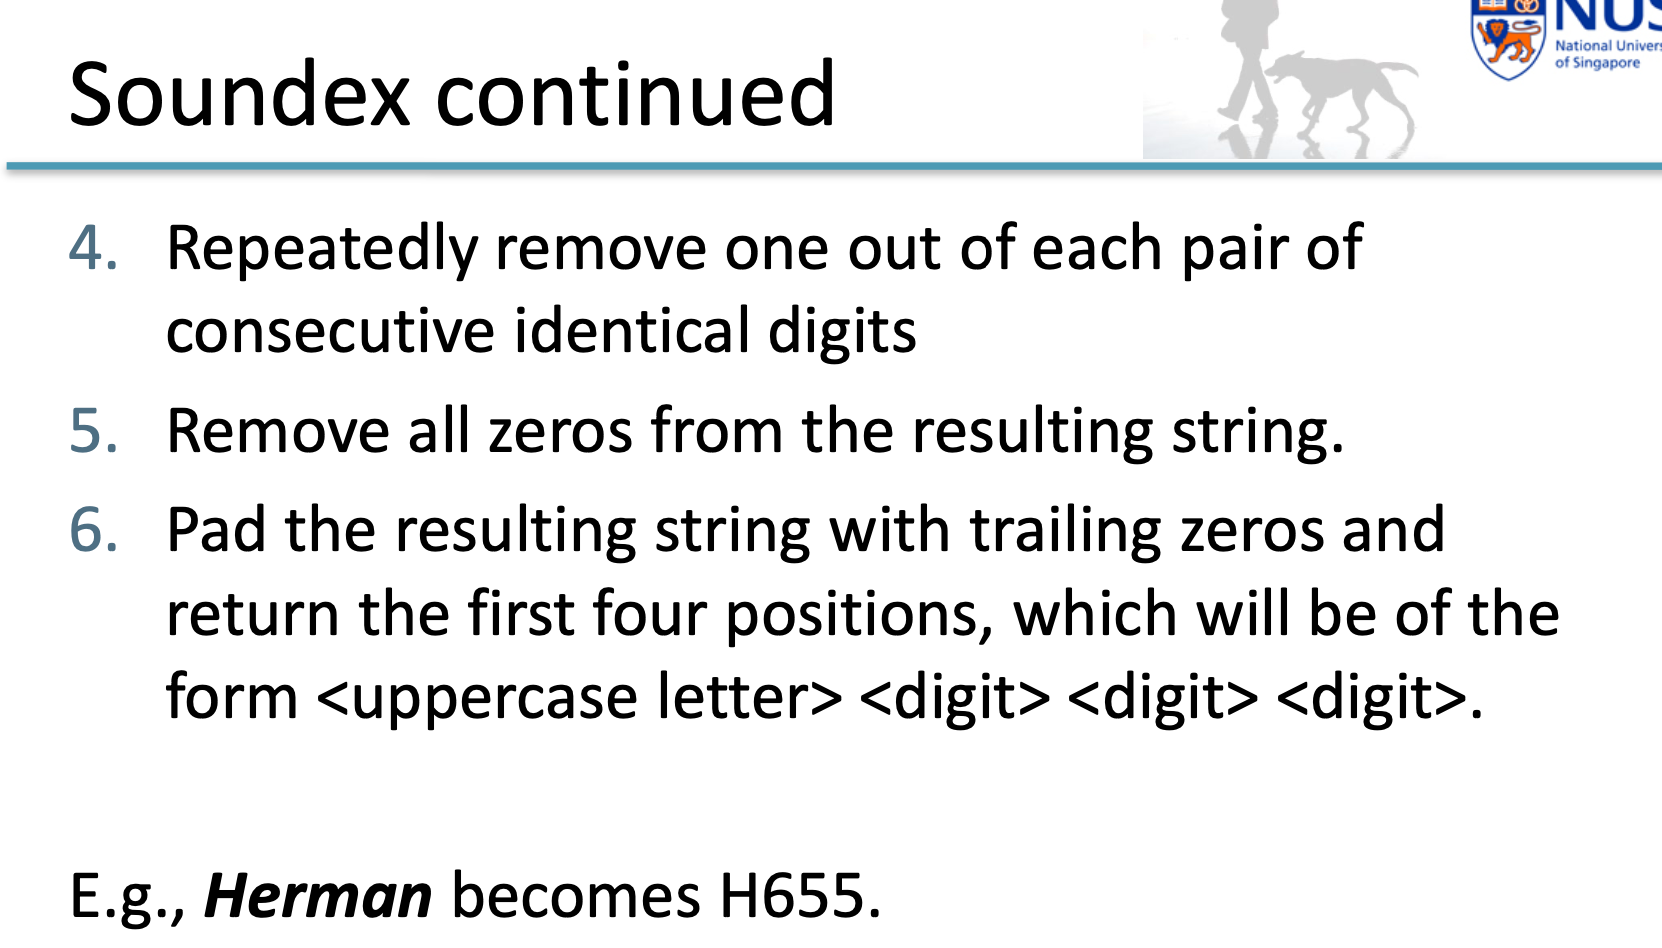
\includegraphics[height=5cm]{ir3}\\
\subsection*{Stop words removal}
cause some phrase search to be less precise
\subsection*{Permuterm index}\\
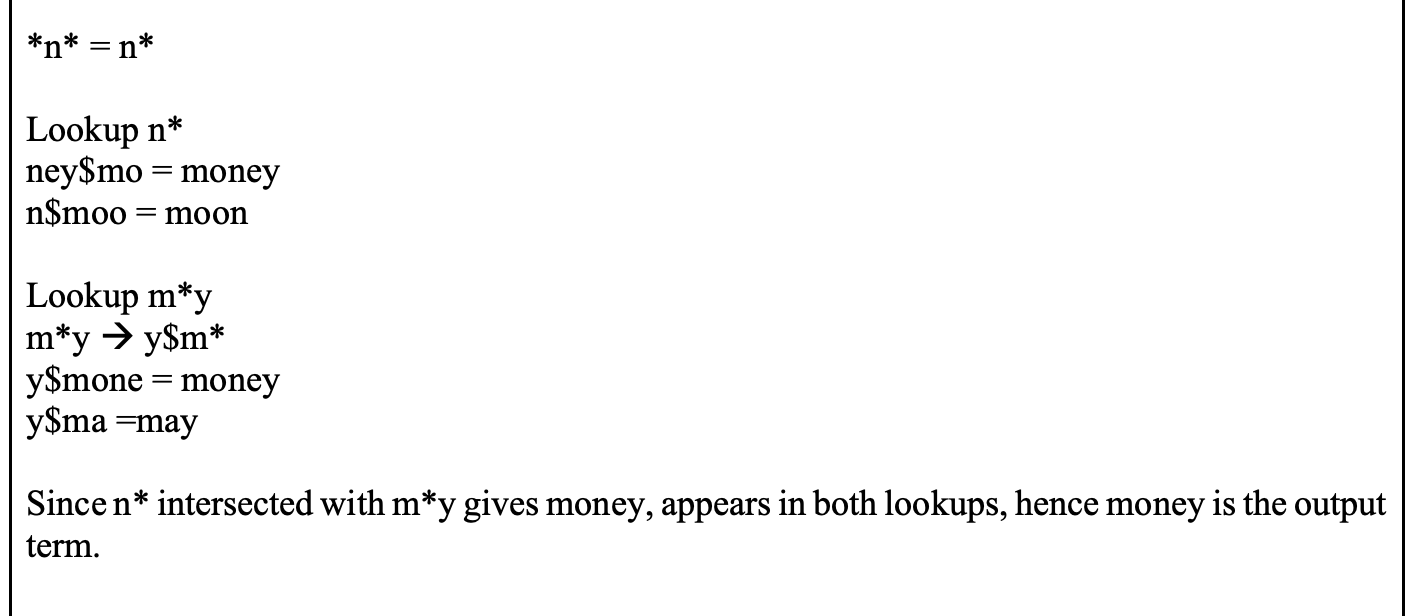
\includegraphics[height=5cm]{ir6}\\
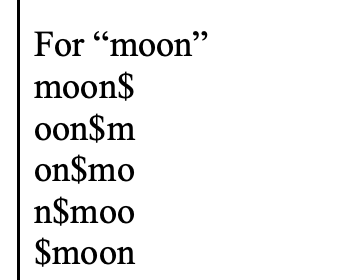
\includegraphics[height=2cm]{ir7}
\subsection*{Cluster pruning}
leaders are chosen at random, and followers are precomputed\\\\
a document will be the follower of the leader whose cosine similarity with the document is the highest

\subsection*{To cut down index size}
Remove stop words 200MB savings\\
VB encoding during SPIMI block splitting stage 400MB savings\\
remove CSS/JS/HTML/Chinese characters, terms with only punctuations
posting compression (gap encoding)
\end{multicols*}

\end{document}
